\documentclass[amssymb,twocolumn,aps]{revtex4}

% allows special characters (including æøå)
\usepackage[utf8]{inputenc}
%\usepackage [norsk]{babel} %if you write norwegian
\usepackage[english]{babel}  %if you write english

\usepackage{physics,amssymb}  % mathematical symbols (physics imports amsmath)
\usepackage{graphicx}         % include graphics such as plots
\usepackage{xcolor}           % set colors
\usepackage{float}			  % force placement of tables and figures
\usepackage{algorithm}
\usepackage{algpseudocode}
\usepackage{placeins}
\usepackage{booktabs}
\usepackage{array}
\usepackage{hyperref}         % automagic cross-referencing 

\bibliographystyle{apsrev4-2}
\bibliography{biblio}

\begin{document}


\title{Report Template \\
    \normalsize FYS-STK3155 - Project 1}
\date{\today}
\author{Student}
\affiliation{University of Oslo}

%\newpage


\begin{abstract}
    The abstract gives the reader a quick overview of what has been done and the most important results. Try to be to the point and state your main findings. It could be structured as follows:
    \begin{itemize}
        \item Short introduction to topic and why its important
        \item Introduce a challenge or unresolved issue with the topic (that you will try to solve)
        \item What have you done to solve this
        \item Main Results
        \item The implications
    \end{itemize}
\end{abstract}

\maketitle
\section{Introduction}


Transforming data into knowledge has a long history in science, exemplified  as early as in the 16$^{\text{th}}$ century when Johannes Kepler discovered the empirical laws of planetary motion\cite{patrec} by using Tycho Brahe's astronomical observations of the planet Mars \cite{Yamahata_2024}. Because real-world phenomena rarely can be described by closed-form analytical expressions, we collect data in order to approximate a general relationship between the inputs and outputs
$$y = f(x) + \epsilon,$$
where $\epsilon$ is noise. This is the foundational idea of \textit{supervised learning}, where models are trained on known input and output to capture the underlying relationship in order to predict outputs for unseen inputs \cite{rasch5}.

A reasonable assumption is that through supervised learning, our model should be able to reproduce our observations exactly, while being able to approximate new, unseen observations. \textit{Interpolation} gives us the framework for estimating $f(x)$ within a dataset. \textit{Polynomial interpolation} seeks to fit a polynomial model $p(x)$ such that $$p_d(x_i) = f(x_i),\quad i\in \{0,1, 2\dots,  n\},$$ where $_d(x)$ is a polynomial degree $n-1$ or higher, passes through $n$ data in order to estimate intermediate values\cite{johau1}. The Runge phenomenon, depicted in Figure~\ref{fig:rungesfunction} with the corresponding error in Table~\ref{tab:runge_error}, illustrates the limitations of this method, with the error $$\max_{x \in [-1,1]} \lvert f(x) - p(x) \rvert, $$ increasing when the number of equally spaced data increases, and subsequently the degree of polynomial, because of the oscillation that occurs at the endpoints. This is reminiscent of overfitting. A solution within interpolation could be \textit{piecewise polynomial interpolation}, where we use a collection of lower degree polynomial interpolants \cite{johau2}, to model the behaviour in intervals,
\begin{equation*}
    S(x)=
    \begin{cases}
        p_0(x),     & x_0 \le x \le x_1     \\
        p_1(x),     & x_1 \le x \le x_2     \\
        \vdots      & \vdots                \\
        p_{n-1}(x), & x_{n-1} \le x \le x_n
    \end{cases},
\end{equation*}
to smoothen the oscillation at the endpoints. However, unwanted local oscillations can still occur. This raises the issue of overfitting: how can we fit data accurately while preserving the model’s ability to generalize to unseen data?

Rather than constraining the model to pass directly through seen data, we should find a model that minimizes the error for unseen data. We will frame the problem as a regression task and apply Ordinary Least Squares, Ridge, and Lasso methods to approximate Runge's function $$ f(x) = \frac{1}{1+25x^2},$$ and use the \textit{mean squared error} (MSE) as our cost function. We will use regularization techniques in tandem with hyperparameter tuning for \textit{model selection} and MSE, bootstrap validation, train-test split, and cross validation for \textit{model assessment}\cite{fysml1}.

In section \hyperref[section:methods]{II}, we will present an overview of regression models such as Ordinary Least Squares, Ridge and Lasso, and how these can be implemented with optimization algorithms, such as \textit{gradient descent} with and without \textit{momentum} and \textit{stochastic gradient decent}, and how we can test the model's performance using resampling methods, such as bootstrap and cross-validation.
In section \hyperref[section:results]{III}  we will discuss and present our results, as well as pros and cons of the implemented methods and identify areas of improvement.

\begin{figure}[h]
    \centering
    \includegraphics[width=\linewidth]{Figures/pol_int.png}
    \caption{Runge's function and polynomial interpolants $p_5(x)$ and $p_{11}(x)$.}
    \label{fig:rungesfunction}
\end{figure}

\begin{table}
    \centering
    \begin{tabular}{c | c | c}
        $n$ data & Degree $(n-1)$ & $\max|f(x) - p_{n-1}(x)|$ \\
        \hline
        2        & 1              & $9.61e^{-1}$              \\
        3        & 2              & $6.46e^{-1}$              \\
        4        & 3              & $7.07e^{-1}$              \\
        5        & 4              & $4.38e^{-1}$              \\
        6        & 5              & $4.33e^{-1}$              \\
        7        & 6              & $6.17e^{-1}$              \\
        8        & 7              & $2.47e^{-1}$              \\
        9        & 8              & $1.05e^{0}$               \\
        10       & 9              & $3.00e^{-1}$              \\
        11       & 10             & $1.92e^{0}$               \\
        12       & 11             & $5.57e^{-1}$              \\
        \vdots   & \vdots         & \vdots                    \\
        99       & 98             & $1.65e^{2}$               \\
        \bottomrule
    \end{tabular}
    \caption{Maximum interpolation error $\max |f(x) - p(x)|$ for Runge's function using equally spaced data on $[-1,1]$.}
    \label{tab:runge_error}
\end{table}

\section{Methods}\label{section:methods}
Throughout this article, multiple methods for regression, metrics for evaluating performance, gradient descent and resampling techniques are used, this section is split into four subsections presenting each topic in order. We will first present the relevant regression methods, then go into more detail on how to measure their performance. All of the presented regression models can be optimized using various techniques, as such, the third subsection will tackle gradient descent, before we forth and finally present resampling.

\subsection{Regression}
In this section, three regression methods are presented \textit{ordinary least squares, ridge regression} and \textit{lasso regression}. They will be presented in order and cover both the theoretical basis, algoritmic approach and briefly, our own implementation.

\subsubsection{Ordinary Least Squares}
Ordinary least squares (OLS) is one of the most common methods for fitting linear regression models as it is easy to understand and implement compared to other regression models. Unlike polynomial interpolation, OLS regression does not require the model to match every data point or to use a minimum polynomial degree based on the number of data points. Instead, you select the number of predictors based on fit quality - such as $R^2$ and \textit{mean squared error} (MSE). This flexibility is desirable when estimating non-linear functions such as Runge's as we can approximate the function well without overfitting.


Since MSE is a measure of the lack of fit of the model to the data, the least squares method seeks to find the parameter estimates $\hat{\theta}$ that minimize this cost function, defined as
$$C(\theta)  = \frac{1}{n} \sum_{i=1}^{n} \left( y_i - \hat{y}_i \right)^2.$$
Because the cost function is a quadratic function and $X^TX$ is positive-semidefinite, the cost function is convex and must have a minimum. Setting the derivative with respect to $\theta$ equal to zero, $$\frac{\partial C(\theta)}{\partial \theta} = 0,$$
and solving for $\theta$ gives us the closed-form solution
$$\hat{\theta} = \left( X^T X \right)^{-1} X^T y.$$

An additional motivation for approximating Runge's function with OLS is it's property of unbiasedness: we can use the sample  mean \textit{$\hat{\mu}$ }to estimate $\mu$ \cite{introstat}. Among all unbiased estimates the OLS has the smallest variance according to the Gauss-Markov theorem \cite{hastie1}. We will revisit these points when we discuss the bias–variance trade-off.

In this project we implemented OLS using a self-written python code, following the structure of \hyperref[algorithm:OLS]{Algorithm 1}, using Scikit-Learn's \text{train\_test\_split} \cite{scikit-learn} to split the feature matrix into a test and test dataset. The training set were used to train the model and the test set was used for measuring quality fit on unseen data using MSE and $R^2$. Because the OLS estimators are scale equivariant, meaning if we scale our estimators we still end up with the same predictor, we don't have to scale our design matrix \cite{introstat}.


\begin{algorithm}[H]
    \caption{Ordinary Least Squares}
    \label{algorithm:OLS}
    \begin{algorithmic}[1]
        \State Given data matrix $X \in \mathbb{R}^{n}$, p predictors, targets $y \in \mathbb{R}^n$
        \State Compute design matrix with polynomial features

        $X \in \mathbb{R}^{n \times p}$
        \State Estimate parameters:
        $\hat{\theta} = (X^T X)^{-1} X^T y$
        \State Predictions: $\hat{y} = X \hat{\theta}$
        \State Evaluate quality of fit with MSE and $R^2$
    \end{algorithmic}
\end{algorithm}


\subsubsection{Ridge Regression}

The reason we are not satisfied with least squares estimates is because of it's prediction accuracy \cite{fysml2}. OLS gives us low bias and potentially large variance due to how we calculate the estimators $\hat{\theta}$. Recall
$$\hat{\theta}_{OLS} = (X^TX)^{-1}X^Ty$$
works only if $X^TX$ can be inverted, meaning $det(X^TX) \neq 0$ and $X$ is linearly independent \cite{fysml2}. If the determinant is close to zero, meaning we can compute it's inverse, there will be high variance in our estimates due to small changes in $y$ can cause large swings in $\hat{\theta}$. If our design matrix X has linearly dependent column vectors, $det(X^TX) = 0$, we will not be able to compute $(X^TX)^{-1}$ and in turn our estimators. This is more likely to happen with high-dimensional matrices, such as when we want to approximate Runge's function to a higher order polynomial. To mitigate this we can use Ridge regression.

Ridge regression solves this by imposing a penalty, also known as L2 regularization, to the least squares method \cite{fysml2},
$$X^TX \to X^TX+\lambda I,\quad \lambda \geq 0,$$
where $I$ is the identity matrix and $\lambda$ is the regularization strength. Giving us
$$\hat{\theta}_{Ridge} = (X^TX+\lambda I)^{-1}X^Ty$$
By increasing $\lambda$ we shrink the regression coefficients resulting in fewer extreme outliers and stabilizing the estimates by reducing the variance at the cost of bias \cite{elestat1}. This results in an improvement of the OLS prediction accuracy which we were after.

As shown in Algorithm~\ref{algorithm:Ridge}, Ridge regression extends OLS by \textit{standardizing} the columns of the design matrix and by introducing an L2 penalty to the estimator. We standardize the feature column of the design matrix by subtracting the mean and divide by the standard deviation for each column.
$$X_{scaled} = \frac{X-\mu}{\sigma}$$

The reason for this is that we want the shrinking to be uniform across features. If we did not scale $X$ then large variance features would be shrunk more and the low variance features would be shrunk less  resulting in uneven penalization \cite{introstat1}. Just like we did with ordinary least squares we will explore the

Our Ridge regression code implementation follows the order of operations given in \hyperref[algorithm:Ridge]{Algorithm~\autoref{algorithm:Ridge}}. Similar to our OLS implementation we will use Scikit-Learn for our train/test split and use MSE and $R^2$ as our quality fit measure. As scaling the feature matrix is crucial in Ridge, we used Scikit-Learn's StandardScaler for this. We will compare our results with OLS using the same seed, yielding same inputs and outputs when generating data, so that the results are comparable. In particular, we want to investigate whether the L2 penalty results in a better fit when $X^TX$ is close to zero. Furthermore, we will explore Ridge's dependence on the penalty strength $\lambda$ and degree of polynomial. We will also compare the results using $\theta$ obtained using the closed-loop expression and gradient descent algoritm.

\begin{algorithm}[H]
    \caption{Ridge Regression}
    \label{algorithm:Ridge}
    \begin{algorithmic}[1]
        \State Given $X \in \mathbb{R}^{n}$, p predictors, $y \in \mathbb{R}^n$, penalty $\lambda$
        \State Compute design matrix with polynomial features

        $X \in \mathbb{R}^{n \times p}$
        \State Standardize each column $X$
        \State Estimate parameters:
        $$\hat{\theta} = (X^\top X + \lambda I)^{-1} X^\top y$$
        \State Predictions: $\hat{y} = X \hat{\theta}$
        \State Evaluate quality of fit with MSE and $R^2$
    \end{algorithmic}
\end{algorithm}



\subsubsection{Lasso Regression}

Lasso regression, \textit{Least Absolute Shrinkage and Selection Operator}, is a very similar method to Ridge regression as it introduces a penalty term into the cost function to mitigate the problem of overfitting at higher model complexities \cite{Raschka-et-al-2022}. For Lasso, we use the L1 penalty,

$$||\theta||_1 = \sum^m_{j=1}|\theta_j|,$$

which leads to the Lasso cost function,

$$ C_{Lasso}(\boldsymbol{X}, \theta) = (y - \boldsymbol{X}\theta)^T(y-\boldsymbol{X}\theta) + \lambda ||\theta||_1.$$

Taking the derivative of the cost function with respect to $\theta$ and recalling that the derivative of the absolute value is $\frac{d|\theta|}{d\theta} = sgn(\theta),$, we make two important observations \cite{fysml2}\cite{Hastie-et-al-2009}:

$$\boldsymbol{X}^T\boldsymbol{X} \theta + \lambda sgn(\theta) = 2\boldsymbol{X}^Ty$$

\begin{enumerate}
    \item We cannot obtain a closed form solution for $\hat{\theta}$ as the function is discontinuous at zero.
    \item The L1 penalty is constant and does not scale with the magnitude of the coefficients like the L2 penalty. Consequently, if a coefficient contribution to the cost function is sufficiently small, i.e. less than $\lambda$, it will be driven to zero by the penalty term.
\end{enumerate}

The challenge posed by the first observation can be solved using convex optimization algorithms like gradient decent, which we will come back to in the next section. The second observation results in a form of automatic feature selection, where only the coefficients that contribute to the cost function are retained, while those that don't are driven to zero. This is especially relevant for larger datasets with many parameters. Algorithm \ref{algorithm:Lasso} shows the general structure of Lasso regression.

\begin{algorithm}[H]
    \caption{Lasso Regression}
    \label{algorithm:Lasso}
    \begin{algorithmic}[1]
        \State Given $X \in \mathbb{R}^{n \times p}$, $y \in \mathbb{R}^n$, penalty $\lambda$
        \State Compute design matrix with polynomial features
        \State Standardize each column $X$
        \State Compute the Lasso estimator using a convex optimization method, e.g. gradient descent, see algorithm \ref{algorithm:GD}, \ref{algorithm:GDM} and \ref{algorithm:SGD}:
        \State Predictions: $\hat{y} = X \hat{\theta}$
    \end{algorithmic}
\end{algorithm}


\subsection{Evaluation metrics}
In \textit{supervised learning} we are interested in finding the machine learning algorithm that makes the best prediction on \textit{unseen data} based on the patterns learned from the \textit{seen data} \cite{fysml6}. Since we already know what the response $y$ is given $x$ we can evaluate how good the prediction $\hat{y}$ is. In regression we split our observed data $(x_i, y_i)$ into two batches: training and testing dataset. Usually the test size is 20-30\% of our data. The reason for this is that we want to train a model that makes the best possible prediction, meaning that a too-small train size may fail to capture the underlying pattern. After we have trained our model we can evaluate the performance of the model using our test data. Since our goal is to build a model that can predict future inputs, we evaluate its performance using the test data. To measure performance we use model assessment metrics such as \textit{mean squared error}, \textit{$R^2$} and \textit{bias-variance tradeoff}.

\subsubsection{Mean Squared Error}
One way to quantify how good a model is at predicting is the \textit{mean squared error} (MSE), defined as
$$MSE = \frac{1}{n}\sum_{i=0}^{n-1}(y_i-\hat{y}_i)^2,$$
where $\hat{y}_i$ is the prediction for the \textit{i}th observation. The MSE measures how much the collection of predictions deviates from the true response. A small MSE means that the predictions are on average close to the observations, and a large value corresponds to predictions being on average further away. In other words we can say that MSE is a measure of lack of fit of the mode.

The squaring of the error ($y_i-\hat{y_i}$) ensures that the terms don't cancel each other, making it easier to interpret the result. It also means that large errors get penalized more than small errors, making it more sensitive to outliers. One of the most useful properties is that this leads to a convex quadratic function, which regression models such as \textit{OLS} and \textit{Ridge} optimize to find their optimal estimator $\hat{\theta}$ \cite{introstat3}.

Beyond model assessment, MSE can also be used as a metric for model selection. In Figure~\ref{fig:biasvariancemse} we can see MSE as a function of polynomial degree. Given that we evaluate performance on the test data and that low MSE is desirable, we can choose the model complexity that yields the lowest test MSE.

\begin{figure}[h]
    \centering
    \includegraphics[width=\linewidth]{Figures/biasvariance.png}
    \caption{Training and testing MSE as we vary the polynomial degree for $n$ = 50 using ordinary least squares.}
    \label{fig:biasvariancemse}
\end{figure}

\subsubsection{Bias-variance tradeoff}
\label{sec:bvt}
Recall that we can consider the test MSE as a measure of the lack of fit of the model to the data using linear algebra analysis. To get a deeper understanding of why that is we will use \textit{bias-variance tradeoff} from statistical analysis and the Figure~\ref{fig:biasvariancemse} to get a better intuition.

The characteristic U-curve for the test MSE has in Figure~\ref{fig:biasvariancemse} is the result of two competing statistical properties, the $\textit{bias}^2$ and \textit{variance}. In the context of machine learning models, \textit{bias} refers to the error introduced by approximating a complex function using a much simpler model. For instance, approximating the polynomial $x^2+3x^4+\sqrt{2}x^5$ using a linear model $\theta_0 +\theta_1x$ will result in bias as it does not produce an accurate estimate. Generally more flexible models, e.g. higher polynomial degree, result in less bias \cite{introstat2} as the predictions $\hat{y}$ is closer to $y$. On the other hand, \textit{variance} measures the consistency of our predictor $\hat{y}$ if we estimate it using different subsets of the training data set. If small changes in the training data results in large changes in $\hat{y}$ we say that the model has high variance. Using a feature matrix with high polynomial degrees as our predictors will amplify these changes, resulting in higher variance.

Statistically, without deriving it, the expected error gives the the following bias–variance decomposition
\begin{equation}
    \label{eq:bias_variance}
    \mathbb{E}\!\left[(y - \tilde{y})^2\right]
    =
    \underbrace{\mathbb{E}\!\left[(y - \mathbb{E}[\tilde{y}])^2\right]}_{\text{Bias}[\tilde{y}]}
    +
    \underbrace{\mathbb{E}\!\left[(\tilde{y} - \mathbb{E}[\tilde{y}])^2\right]}_{\text{Var}[\tilde{y}]}
    +
    \underbrace{\sigma^2}_{\text{Noise variance}}
\end{equation}


Now we are better equipped to understand the behavior of the test error in Figure~\ref{fig:biasvariancemse}, as model complexity is varied. In Figure~\ref{fig:biasvar} we have used this decomposition to plot the bias and variance as a function of polynomial degree. Using what we know about bias and variance we can say that bias decreases and variance increases as we increase the model complexity. This means that we cannot decrease the bias and variance as the same time, thus the name \textit{bias-variance tradeoff}.

When we have high bias we say that our model is \textit{underfit} because our model is not complex enough to capture the underlying patterns in the data. In contrast, \textit{overfitting} is when a model is too complex to capture the pattern \cite{rasch3}.

\begin{figure}[h]
    \centering
    \includegraphics[width=\linewidth]{Figures/biasvar.png}
    \caption{$Bias^2$, Variance and noise as we vary the polynomial degree for $n$ = 50 using ordinary least squares.}
    \label{fig:biasvar}
\end{figure}


\FloatBarrier
\subsubsection{$R^2$ Score}

The coefficient of determination ($R^2$) is an alternative measure of fit. Where the MSE measures how far away our prediction is on average, the $R^2$ measures the fraction of the response variance that can be explained by the model \cite{rasch4} \cite{fysml7}. To calculate $R^2$, we use

\begin{align}
    R^{2} & = 1 - \frac{\sum_{i=0}^{n-1} (y_i - \hat{y}_i)^2}{\sum_{i=0}^{n-1} (y_i - \bar{y})^2}                                   \\
          & =  \frac{ \sum_{i=0}^{n-1} (y_i - \bar{y})^2- \sum_{i=0}^{n-1} (y_i - \hat{y}_i)^2}{\sum_{i=0}^{n-1} (y_i - \bar{y})^2}
\end{align}
where $\bar{y}$ is the mean value of y. The denominator in equation (1) is the \textit{total sum of squares} (TSS), measuring the total variance in our target before regression is performed, and the numerator is the \textit{residual sum of squares} (RSS), measuring the variability that is unexplained after performing the regression \cite{introstat4}. For intuition we can look at equation (2) as
$$R^2 \approx \frac{\text{Variance explained by the regression line}}{\text{Total variance around the mean}}.$$
$R^2$ takes a value between 0 and 1. An $R^2$ score of 1 indicates that the regression line explains all of the variability, meaning a perfect fit. Contrarily, an $R^2$ of 0 means the regression like explains none of the variability.

Similar to MSE, the $R^2$ can also be used as a metric for model selection. Given that we evaluate performance on the test data and that high $R^2$ score is desirable, we can choose the model complexity that yields the highest test $R^2$.


\subsection{Gradient decent}
\label{sec:gd}

Recall that we found the values of $\hat{\theta}$ that minimize the cost function using closed-form solutions. As pointed out in \cite{fysml3}, computing predictor estimates using closed-form solutions can become impractical in high-dimensional settings due to the computational demands of inversion of the feature matrix. Instead, we must use numerical methods to compute the minimum. One of these methods is the \textit{gradient descent}.

Gradient descent is an iterative algorithm that moves on the curve, or surface as seen in \autoref{fig:gd}, in the opposite direction of the gradient $$\nabla_\theta C(\theta),$$ until a local or global loss minimum is reached. Algorithm \autoref{algorithm:GD} describes how we compute the estimators. In each iteration, we take a step in the steepest descent, where the step size is determined by the gradient evaluated at that point and the learning rate, $\eta$,$$\theta^{n+1} = \theta^n - \eta\nabla_\theta(\theta^n).$$
Since the MSE is convex, convergence is guaranteed given enough iterations, the iterations approach the estimator $\hat{\theta}$ where the gradient  term vanishes, $$\nabla_\theta C(\hat{\theta}) = 0.$$

However, this method has some drawbacks as it can lead to slow convergence or even failure to converge as it takes large steps in the direction of steepest descent and small steps where the gradient is shallow. Gradient descent is also computationally heavy for large dataset and higher-dimensional feature matrices \cite{fysml4}, as each iteration requires computing the gradient over the entire dataset, making it slow and inefficient at scale \cite{rasch1}. Depending on our initial guess for $\theta$ and learning rate, there is a possibility that we converge to a local minima or saddle point when using this algorithm on non-convex cost functions, introducing uncertainty in the final results. To overcome these challenges, variants of gradient descent such as with \textit{momentum} and \textit{stochastic gradient descent} have been developed to accelerate convergence and handle large datasets more efficiently

Algorithm \ref{algorithm:GD} takes us through our code implementation for GD.

\begin{algorithm}[H]
    \caption{Gradient Descent}
    \label{algorithm:GD}
    \begin{algorithmic}[1]
        \State Given learning rate $\eta$, iterations $T$, initial parameters $\theta^{(0)}$
        \For{$t = 0,1,\dots,T-1$}
        \State Compute gradient: $\nabla_\theta C(\theta^n)$
        \State Update parameters: $\hat{\theta} \gets \theta^{n+1} = \theta^n - \eta\nabla_\theta(\theta^n)$
        \EndFor
        \State Predictions: $\hat{y} = X \hat{\theta}$
    \end{algorithmic}
\end{algorithm}


\begin{figure}[H]
    \centering
    \includegraphics[width=1\linewidth]{Figures/gradient_descent.png}
    \caption{Contour plot of the MSE cost function with GD path from the starting point $(\theta_0, \theta_1)$ = (1,4).}
    \label{fig:gd}
\end{figure}



\subsubsection{Gradient Descent with Momentum}

Gradient descent with momentum can be imagined as rolling a physical ball down a slope—the ball is affected by gravity, thus it accelerates and gains velocity and momentum down the slope. The steeper the slope, the greater the momentum becomes. Even if the slope becomes less steep or changes direction, the ball will "remember" its previous momentum, helping it overcome small local minima and dampen oscillations in narrow valleys.

One of the main drawbacks of vanilla gradient descent is that the step size and direction only depend on the gradient at that point and the learning rate, $\eta$. As the gradient approaches a value close to zero, the step size also converges towards zero, even though this minimum might not be the global minimum. This is especially true for datasets that result in noisy or small but consistent gradients \cite{Goodfellow-et-al-2016}.

To mitigate this and to accelerate learning, \textit{momentum} or "memory" can be introduced. This method takes all or a selection of previous gradients into account when calculating the step size and direction. We call this the \textit{velocity} ($v$) of the gradient,

$$v^{(n+1)} = \alpha v^{(n)} - \eta \boldsymbol{g}^{(n)},$$

where $\alpha$ is the momentum parameter, and

$$\boldsymbol{g}^{(n)} = \nabla_\theta C(\theta^{(n)}).$$

From this we can see that the cumulative impact behaves like an exponentially decaying moving average of the previous gradients and is dependent on the momentum parameter $\alpha$. Typical values for $\alpha$ include $0.5$, $0.9$ and $0.99$ \cite{Goodfellow-et-al-2016}, where larger values retain more of the previous gradients. Algorithm \ref{algorithm:GDM} outlines how GDW could be implemented.

\begin{algorithm}[H]
    \caption{Gradient Descent with Momentum (GDM)}
    \label{algorithm:GDM}
    \begin{algorithmic}[1]
        \State Given learning rate $\eta$, momentum parameter $\alpha$, initial parameters $\theta^{(0)}$, initial velocity $v^{(0)} = 0$
        \While{stopping criterion not met}
        \State Compute gradient: $\boldsymbol{g}^{(n)} \leftarrow \nabla_\theta C(\theta^{(n)})$
        \State Compute velocity update: $v^{(n+1)} \leftarrow \alpha v^{(n)} - \eta \boldsymbol{g}^{(n)}$
        \State Update parameters: $\theta^{(n+1)} \leftarrow \theta^{(n)} + v^{(n+1)}$
        \EndWhile
    \end{algorithmic}
\end{algorithm}

Our own implementation follows this algorithm closely - taking the training part of the design matrix and $y$ function as user specified inputs, while using default values for $\alpha=0.9, \eta=0.01$, \textit{[number of iterations]=1000 and [$\theta$ change tolerance]=$10^{-6}$}. We utilize numpy's \cite{2020NumPy-Array} built-in array functionality to for matrix and vector operations and return the optimal $\theta$ value found.


\subsubsection{Stochastic gradient decent}


The vanilla gradient descent method is sometimes referred to as full batch gradient descent because it iterates through the whole dataset. As we discussed in \autoref{sec:gd}, running gradient descent on very large datasets can be computationally costly, since we need to reevaluate the whole dataset at each iterations. A widely used  alternative is stochastic gradient descent (SGD) with mini-batches, denoted as $B_k$, which generates randomly sampled subsets of the data to approximate the gradient, at each iteration $$ \nabla_\theta C(\theta) \approx \sum_{i\in B_k} \nabla_\theta C_i (x_i,\theta), \quad k\in\{1,2, \dots , n/M\}.$$
The number of batches, $k$, is determined by the number of data data points $n$  and the size of our batches $M$.

Substituting our new cost function in the vanilla algorithm yields $$\theta^{n+1} = \theta^n - \eta\sum_{i\in B_k} \nabla_\theta C_i (x_i,\theta),$$
where $k$ is picked at random with equal probability \cite{fysml5}. Each gradient requires $M$ computations, whereas in the gradient descent which we did $n$ computations, saving us $n - M$ calculations per iteration. This is what makes this algorithm efficient. In order to give the full exposure of the dataset we iterate over all the number of batches, also known as an \textit{epoch}. One epoch equates to $n/M$ steps, making one epoch insufficient for reaching the local minima, therefore we rely on iterating multiple epochs of training.

In \autoref{fig:sgd}, we extend \autoref{fig:gd} by adding the trajectory of SGD, which illustrates how the path becomes noisy due to the random sampling, which is beneficial for nonlinear cost function as there is a possibility of "wiggling" out of saddle points.

\begin{figure}[h]
    \centering
    \includegraphics[width=1\linewidth]{Figures/gd_sgd.png}
    \caption{Contour plot of the MSE cost function with GD and SGD path from the starting point $(\theta_0, \theta_1)$ = (1,4).}
    \label{fig:sgd}
\end{figure}



\begin{algorithm}[H]
    \caption{Stochastic Gradient Descent (SGD)}
    \label{algorithm:SGD}
    \begin{algorithmic}[1]
        \State Given learning rate $\eta$, number of epochs $E$, mini-batch size $M$, initial parameters $\theta^{(0)}$
        \For{$e = 1,2,\dots,E$}
        \State Shuffle the training data
        \For{each $B_k$} \Comment{$n/M$  per epoch}
        \State Compute stochastic gradient: $\sum_{i\in B_k} \nabla_\theta C_i (x_i,\theta)$
        \State Update parameters: $$\theta^{n+1} = \theta^n - \eta\sum_{i\in B_k} \nabla_\theta C_i (x_i,\theta),$$
        \EndFor
        \EndFor
        \State $\hat{\theta} \gets \theta^{\text{final}}$
        \State Predictions: $\hat{y} = X \hat{\theta}$
    \end{algorithmic}
\end{algorithm}



\subsection{Resampling}

In some cases our data might be limited to few data points or experiments that
are hard or time-consuming to reproduce. In these cases \textit{resampling}
methods could be used to "generate" new datasets. Using resampling, we repeatedly
draw samples from the given dataset and use these samples to obtain additional
information about the performance of our model \cite{fysml1} \cite{Hastie-et-al-2009}
\cite{murphy1}.

Here we will focus on two commonly used resampling techniques \cite{fysml1}:
\textit{bootstrapping} and \textit{k-fold cross-validation}. We will first apply
the bootstrap method to our OLS model to study the \textit{bias-variance tradeoff}.
We will then use k-fold cross-validation on OLS, Ridge and Lasso regression to
evaluate and compare the performance across models. Both methods are described in more detail in the following subsections.


\subsubsection{Bootstrap}
Suppose we have a training dataset $Z = (z_1, z_2, \dots, z_N)$, and gather $N$ number of samples $B$ times, with replacement, giving us $B$ bootstrapped datasets with $N$ samples. For each of these datasets we can compute the estimator $\hat{\theta}^*$ \cite{fysml1} \cite{Hastie-et-al-2009}.

Given enough bootstrapped datasets, we can apply the central limit theorem (CLT), which states that for a sufficiently large sample size, the distribution of the sample mean approaches a normal distribution. This, in turn, allows us to make an estimation of the best fitting estimator by looking at the mean $\hat{\theta}^*$ \cite{fysml1}. An example of bootstrapping using a simple dataset can be seen in figure \ref{fig:boot_ex}.


\begin{figure}[h]
    \centering
    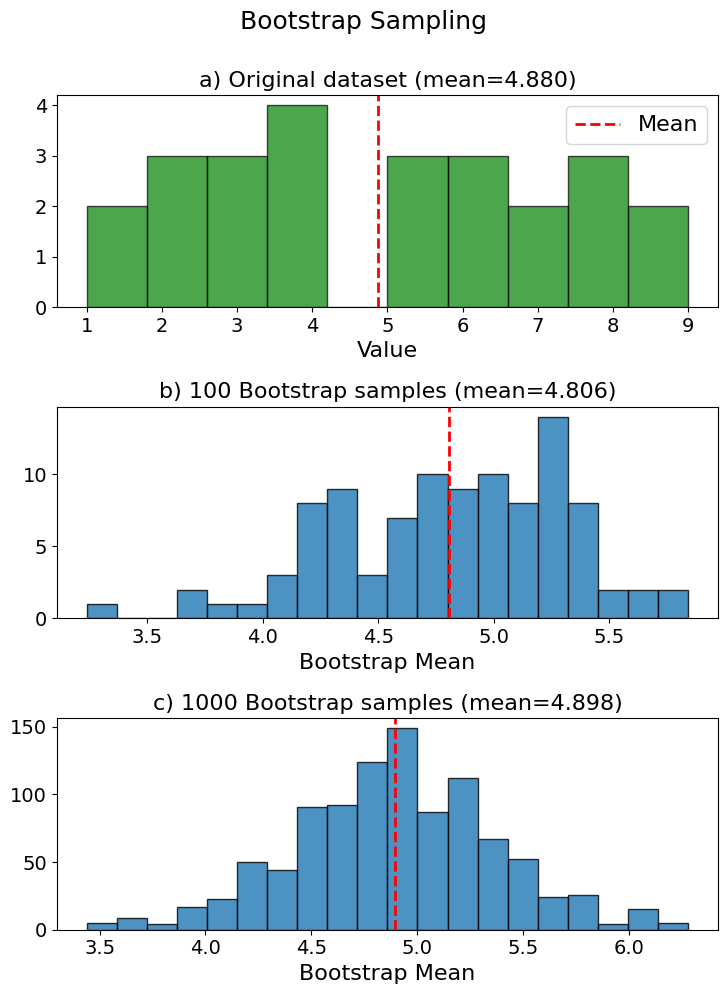
\includegraphics[width=1\linewidth]{Figures/Bootstrap.png}
    \caption{Histograms of a) the original values of the dataset, b) the sampled means of 100 bootstraps, and c) the sampled means of 1000 bootstraps. The original dataset consists of 25 numbers between zero and nine. Each bootstrap samples 25 times with replacement from the original dataset per bootstrap.}
    \label{fig:boot_ex}
\end{figure}

Our bootstrap algorithm takes advantage of the scikit-learn \textit{resample} function \cite{scikit-learn} to resample given datasets in a consistent way. We wrap this function into our own function where we specify the number of samples per bootstrap and number of bootstraps, returning an array of arrays containing the bootstrapped datasets.


\subsubsection{Cross-validation}

In some cases, test data is scarce or unavailable and estimating the test MSE becomes difficult \cite{introstat}. In addition to this, splitting the dataset into training and testing data is generally done randomly. This can, however, lead either subset having an unproportionate amount of outliers which could affect the estimated model \cite{fysml1}. To mitigate both of these challenges, k-fold cross validation splits the data into $K$ \textit{folds}, without replacement \cite{Raschka-et-al-2022}. For each fold, we then train on all folds except k'th, before testing out model on the k'th fold, repeating for $k \in \{1, \dots, K\}$ \cite{murphy1} and combine the estimated error for each step \cite{Hastie-et-al-2009}. This means that we can both estimate the test MSE using the training data, as well as smoothing any potential extremes.
As discussed in \cite{Hastie-et-al-2009} and \cite{Raschka-et-al-2022}, the typical number of folds is five or ten, which corresponds to 20\% and 10\% of the data being used for testing respectively, with ten being the optimal number in many situations. If we choose $K = N$, where N is the total number of samples, we get what is called \textit{leave-one-out cross-validation} (LOOCV). In this case we train on $N - 1$ data points and test on one remaining \cite{Raschka-et-al-2022}, completely eliminating the randomness inherit to dividing the data into subsets as each sample gets its turn as the test sample.

While implementing cross-validation from scratch is relatively straight forward, we choose to leverage the existing functionality of scikit-learn \cite{scikit-learn}. In practice, this means using two functions to define the folds - \texttt{KFold(N)} and \texttt{LeaveOneOut()}, which generates indexes to split the input data into test and training data using $N$ folds, or $N-1$ folds respectively. The split data is then run through our existing regression method functions before returning the results.


\subsection{Use of AI tools}

It is both fitting and amusing that while presenting, implementing and discussing some of the groundwork for machine learning and AI, that we ourselves use these tools to complete this project. Throughout the project period, both ChatGPT\cite{openai2025chatgpt} and Claude AI\cite{anthropic2025claude} have been used. Our main use case has been debugging and altering existing Python and \LaTeX code. However, they have also been used to give suggestions on how to structure our report and as a spellchecker. In the case of Claude AI, all relevant lecture notes and Jupyter notebooks were used as \textit{project knowledge}\cite{anthropic2025projects} and formed the knowledge basis for all interactions related to the project - searching this data first, before checking other sources.

While it is tempting to save time and effort by using these tools to produce the majority of content in this project, we feel like this neither enhances our learning nor necessarily leads to a good report and code. As awesome as these tools can be, they have limitations in occasional hallucinations and misunderstandings, and generally need to be verified against other sources. As such, all text and code used in this project has been produced by us, based on our own understanding of the topics, with available AI tools serving as supporting tools.



\section{Results and Discussion}\label{section:results}
We defined the data gathering process as $$y= f(x) + \epsilon, \qquad \epsilon \sim \mathcal{N}(0,\,\sigma^2),$$
where $\epsilon$ is a normally distributed noise with mean zero and variance $\sigma^2$. As shown in Equation~\ref{eq:bias_variance} in Section~\ref{sec:bvt}, the total expected error contains an irreducible component due to this noise. We can observe the impact this noise has on our metrics, MSE and $R^2$, in  Figure~\ref{fig:noisecomp}. As expected, noise degrades the quality of the fit, by increasing the MSE and reducing the $R^2$ score. Our data was generated using gaussian noise $\epsilon \sim \mathcal{N}(0,\,1)$ to reflect real-world measurement error. Keep this in mind when interpreting our results going forward.

\begin{figure}[h]
    \centering
    \includegraphics[width=\linewidth]{Figures/Discussion/Plots/OLS_noise_comparison.png}
    \caption{MSE and $R^2$ for Runge's function using OLS with $\epsilon = 0$ and $\epsilon = 0.1$, $x\in[-1,1]$.}
    \label{fig:noisecomp}
\end{figure}

We started out by approximating Runge's function using ordinary least squares regression analysis using polynomials as our predictors. In the case of polynomial interpolation, see Figure~\ref{fig:rungesfunction}, we saw that the model was dependent on the number of data points, and as a consequence the polynomial degree. Similarly, we should expect that the OLS model's is influenced by these factors to a certain extent.

Through hyperparameterization resulted in Figure~\ref{fig:OLS_n_poly}. From this plot, we made the following observerations: With few data ($n\in [5,15]$), simpler models are preferable, while larger sample sizes  ($n\in[40,50]$) suggest that increasing polynomial degree improves and stabilizes performance. There is also a high error region for $20\leq n \leq 35$, indicating that ($X^TX$) is nearly singular, which leads to unstable estimators.

\begin{figure}[h]
    \centering
    \includegraphics[width=\linewidth]{Figures/Discussion/Plots/OLS_heatmap_n_vs_poly.png}
    \caption{MSE as a function of polynomial degree and number of data points.}
    \label{fig:OLS_n_poly}
\end{figure}

Based on the preliminary analysis in Figure~\ref{fig:OLS_n_poly}, we selected the $n=50$ column for further analysis, as it yielded stable performance. We then evaluated the model's performance using both MSE and $R^2$. Figure~\ref{fig:OLS_MSE} shows both test MSE and test $R^2$, indicating quality fit for higher degree polynomials. However, beyond polynomial degree 12, we observe diminishing returns with indications of overfitting as both $R^2$ and MSE performs worse for polynomial degree 15. Given these observations, models with polynomial degrees between 6 and 14 are good candidates for our final model. However, the differences in performance among the candidate models are marginal, making it difficult to distinguish which polynomial degree provides the best overall fit. To gain further insight we turn to an analysis of the OLS coefficients and bias-variance tradeoff.
\begin{figure}[h]
    \centering
    \includegraphics[width=\linewidth]{Figures/Discussion/Plots/OLS_mse_r2.png}
    \caption{OLS model performance for $n=50$ across polynomial degrees, showing both MSE and $R^2$ for training and test data.}
    \label{fig:OLS_MSE}
\end{figure}

In Figure~\ref{fig:coef} we can see the magnitude of the coefficients growing rapidly as the degree of the polynomial increases, especially for higher order polynomials. Just as we identified regions of numerical instability in Figure~\ref{fig:OLS_n_poly}, we can see that the coefficients $\theta_8 -\theta_{12}$ for higher order polynomials indicate the same. The bias-variance tradeoff analysis in Figure~\ref{fig:biasvar} suggest that polynomial degree of 8 offers the best balance between bias and variance. This observation is supported in the coefficient plot as this polynomial degree is numerically stable.

\begin{figure}[h]
    \centering
    \includegraphics[width=\linewidth]{Figures/Discussion/Plots/OLS_theta.png}
    \caption{Magnitude of OLS coefficients as a function of polynomial degree for $n=50$. Increasing coefficient magnitude at higher degrees indicates numerical instability and overfitting.}
    \label{fig:coef}
\end{figure}

Numerical instability in OLS, evident in Figure~\ref{fig:OLS_n_poly} and Figure~\ref{fig:coef}, was our motivation for implementing Ridge, In order to get comparable results, we used a fixed seed in our code, replicating inputs-output pairs. In Figure~\ref{fig:ridgehm} and Figure~\ref{fig:ridgetheta} we can see the L2 penalty  slightly damps the spikes. The reason for this is that we used the regularization strength that gave us the column with the lowest MSE in Figure~\ref{fig:pollam}, which was $\lambda=1e^{-5}$. With $\lambda$ is close to zero, meaning Ridge behaves almost identically to OLS, suggests that OLS already captures the underlying relationship well for this dataset.


% Ridge MSE R^2?

\begin{figure}[h]
    \centering
    \includegraphics[width=\linewidth]{Figures/Discussion/Plots/Ridge_heatmap_n_vs_poly.png}
    \caption{MSE as a function of polynomial degree and number of data points, with $\lambda = 1e^{-5}$.}
    \label{fig:ridgehm}
\end{figure}
\begin{figure}[h]
    \centering
    \includegraphics[width=\linewidth]{Figures/Discussion/Plots/Ridge_theta.png}
    \caption{}
    \label{fig:ridgetheta}
\end{figure}
\begin{figure}[h]
    \centering
    \includegraphics[width=\linewidth]{Figures/Discussion/Plots/ridge_heatmap_poly_vs_lambda.png}
    \caption{MSE as a function of polynomial degree and $\lambda$, with $n=50$}
    \label{fig:pollam}
\end{figure}
\begin{figure}[h]
    \centering
    \includegraphics[width=\linewidth]{Figures/Discussion/Plots/eta_heatmap.png}
    \caption{caption}
    \label{fig:}
\end{figure}


Figures \ref{fig:lasso_mse_gd} and \ref{fig:lasso_mse_gdm} show the result of applying Lasso regression using vanilla gradient descent and GD with momentum respectively. We clearly see a reduction in oscillation using momentum as compared to without, both for the MSE and $R^2$-score. We can also observe that the values for MSE and $R^2$-score are generally better with momentum, and that we are able to minimize the cost function at a lower polynomial degree.

\begin{figure}[h]
    \centering
    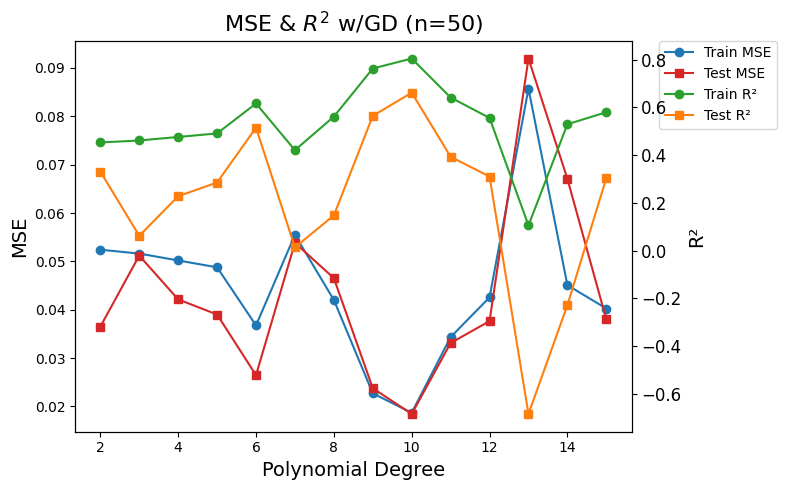
\includegraphics[width=\linewidth]{Figures/Discussion/Plots/Lasso_MSE_R2_GD.png}
    \caption{Plot MSE and $R^2$ score vs polynomial degree for Lasso regression estimate of Rugne's function, using vanilla gradient descent to optimize the estimator.}
    \label{fig:lasso_mse_gd}
\end{figure}

\begin{figure}[h]
    \centering
    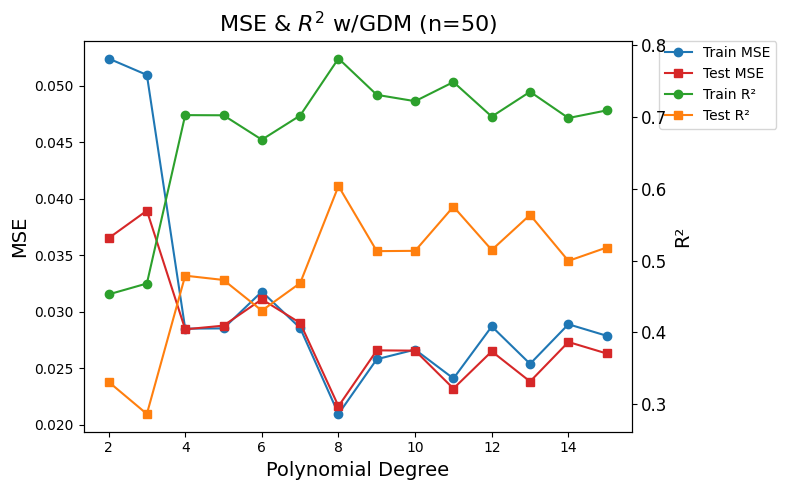
\includegraphics[width=\linewidth]{Figures/Discussion/Plots/Lasso_MSE_R2_GDM.png}
    \caption{Plot MSE and $R^2$ score vs polynomial degree for Lasso regression estimate of Rugne's function, using gradient descent with momentum to optimize the estimator.}
    \label{fig:lasso_mse_gdm}
\end{figure}

As the last step of our analysis we apply cross-validation to all three of our methods using both vanilla GD and GDM to compare their performance using the MSE of their test dataset, The vanilla GD performs slightly worse than the momentum variant, and while there seems to be some oscillations when using momentum, these are within $\approx\pm0.002$ MSE and are not significant. We can observe that across both methods and number of folds lasso regression has the best performance. Ridge performs $\approx$twice as bad as lasso using vanilla GD, while performing almost identically using GDM. The standard OLS approach is consistently worst.

\begin{figure}[h]
    \centering
    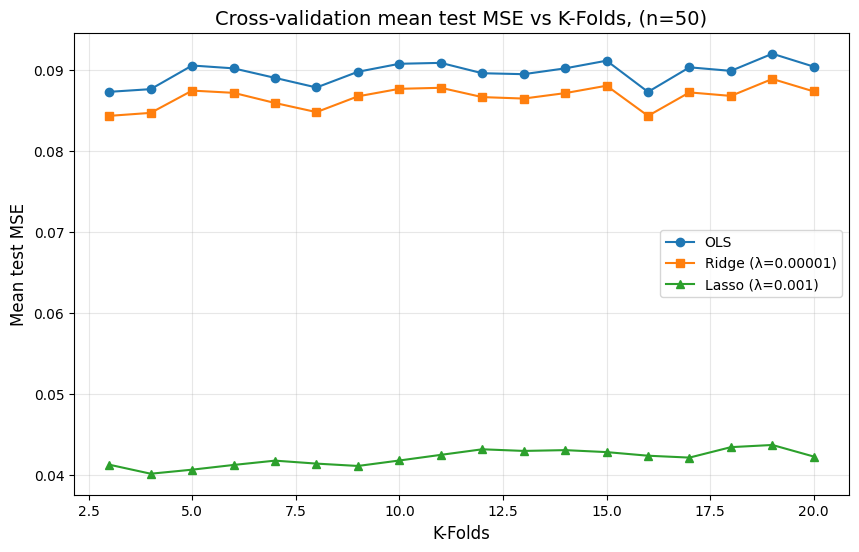
\includegraphics[width=\linewidth]{Figures/Discussion/Plots/CV_comp_GD.png}
    \caption{Comparison of test MSE between OLS, ridge and lasso regression using vanilla gradient descent trying to estimate Rugne's function. Lambda$_{Ridge} = 10^{-5}$, Lambda$_{Lasso} = 10^{-5}$}, polynomial degree = 8, number of folds = 3-20.
    \label{fig:CV_comp_GD}
\end{figure}

\begin{figure}[h]
    \centering
    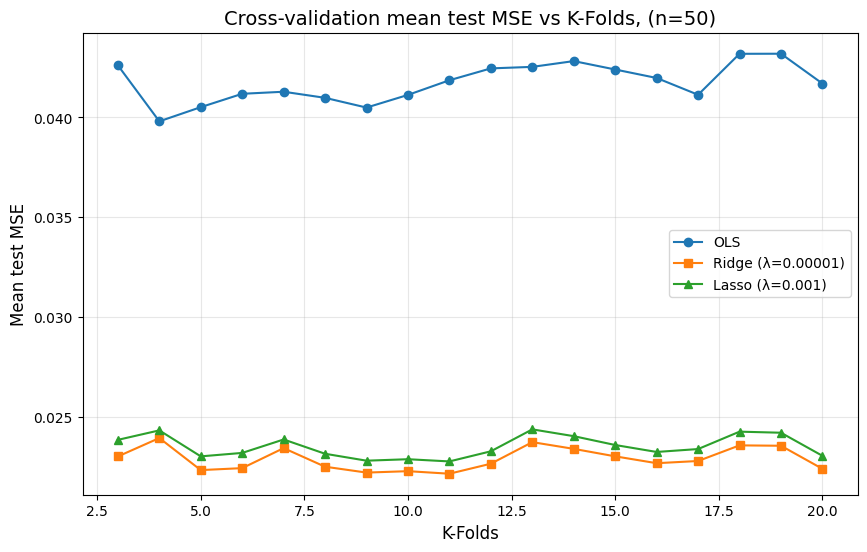
\includegraphics[width=\linewidth]{Figures/Discussion/Plots/CV_comp_GDM.png}
    \caption{Comparison of test MSE between OLS, ridge and lasso regression using gradient descent with momentum trying to estimate Rugne's function. Lambda$_{Ridge} = 10^{-5}$, Lambda$_{Lasso} = 10^{-5}$}, polynomial degree = 8, number of folds = 3-20.
    \label{fig:CV_comp_GDM}
\end{figure}


\section{Conclusion}\label{section:conclusion}

While this report isn't expected to discover anything groundbreaking about how ordinary least squares, ridge regression and lasso regression are implemented and work. It nevertheless presents some of the important background and basics for future projects within machine learning. Throughout this project we have presented  three regression models and discuss various methods for both optimizing and evaluate their respective performance, while comparing the methods to each other. This evaluation and comparison has been done while trying to create a model for Rugne's function - a function known to be hard to interpolate.



\\
Tying the conclusion to the introduction
\begin{itemize}
    \item What have we presented?
    \item What did we find?
    \item What do we think about that?
    \item How did each method perform?
    \item Future work?
\end{itemize}

\begin{itemize}
    \item State your main findings and interpretations
    \item Try to discuss the pros and cons of the methods and possible improvements
    \item State limitations of the study
    \item Try as far as possible to present perspectives for future work
\end{itemize}

\bibliography{biblio}

\end{document}
